\section{ENDF-6 Format}
The ENDF neutron data-files are stored in text files. Each row of the text file is an array of 80 characters. The first 66 characters are formatted depending on the type of the record. Then it follows by 4 characters of material number (MAT), 2 characters of file number (MF), 3 characters of section number (MT), and 5 characters of line number (NS). An illustration of the line structure is shown in Figure \ref{fig:endf-6-record}. The data array at the beginning contains 66 characters whose form depends on the type of the record.  The possibilities are:

\begin{itemize}
\item A string of 66 characters, or
\item Six numbers with each occupying 11 characters.
\end{itemize}

\begin{figure}[h]
\begin{center}
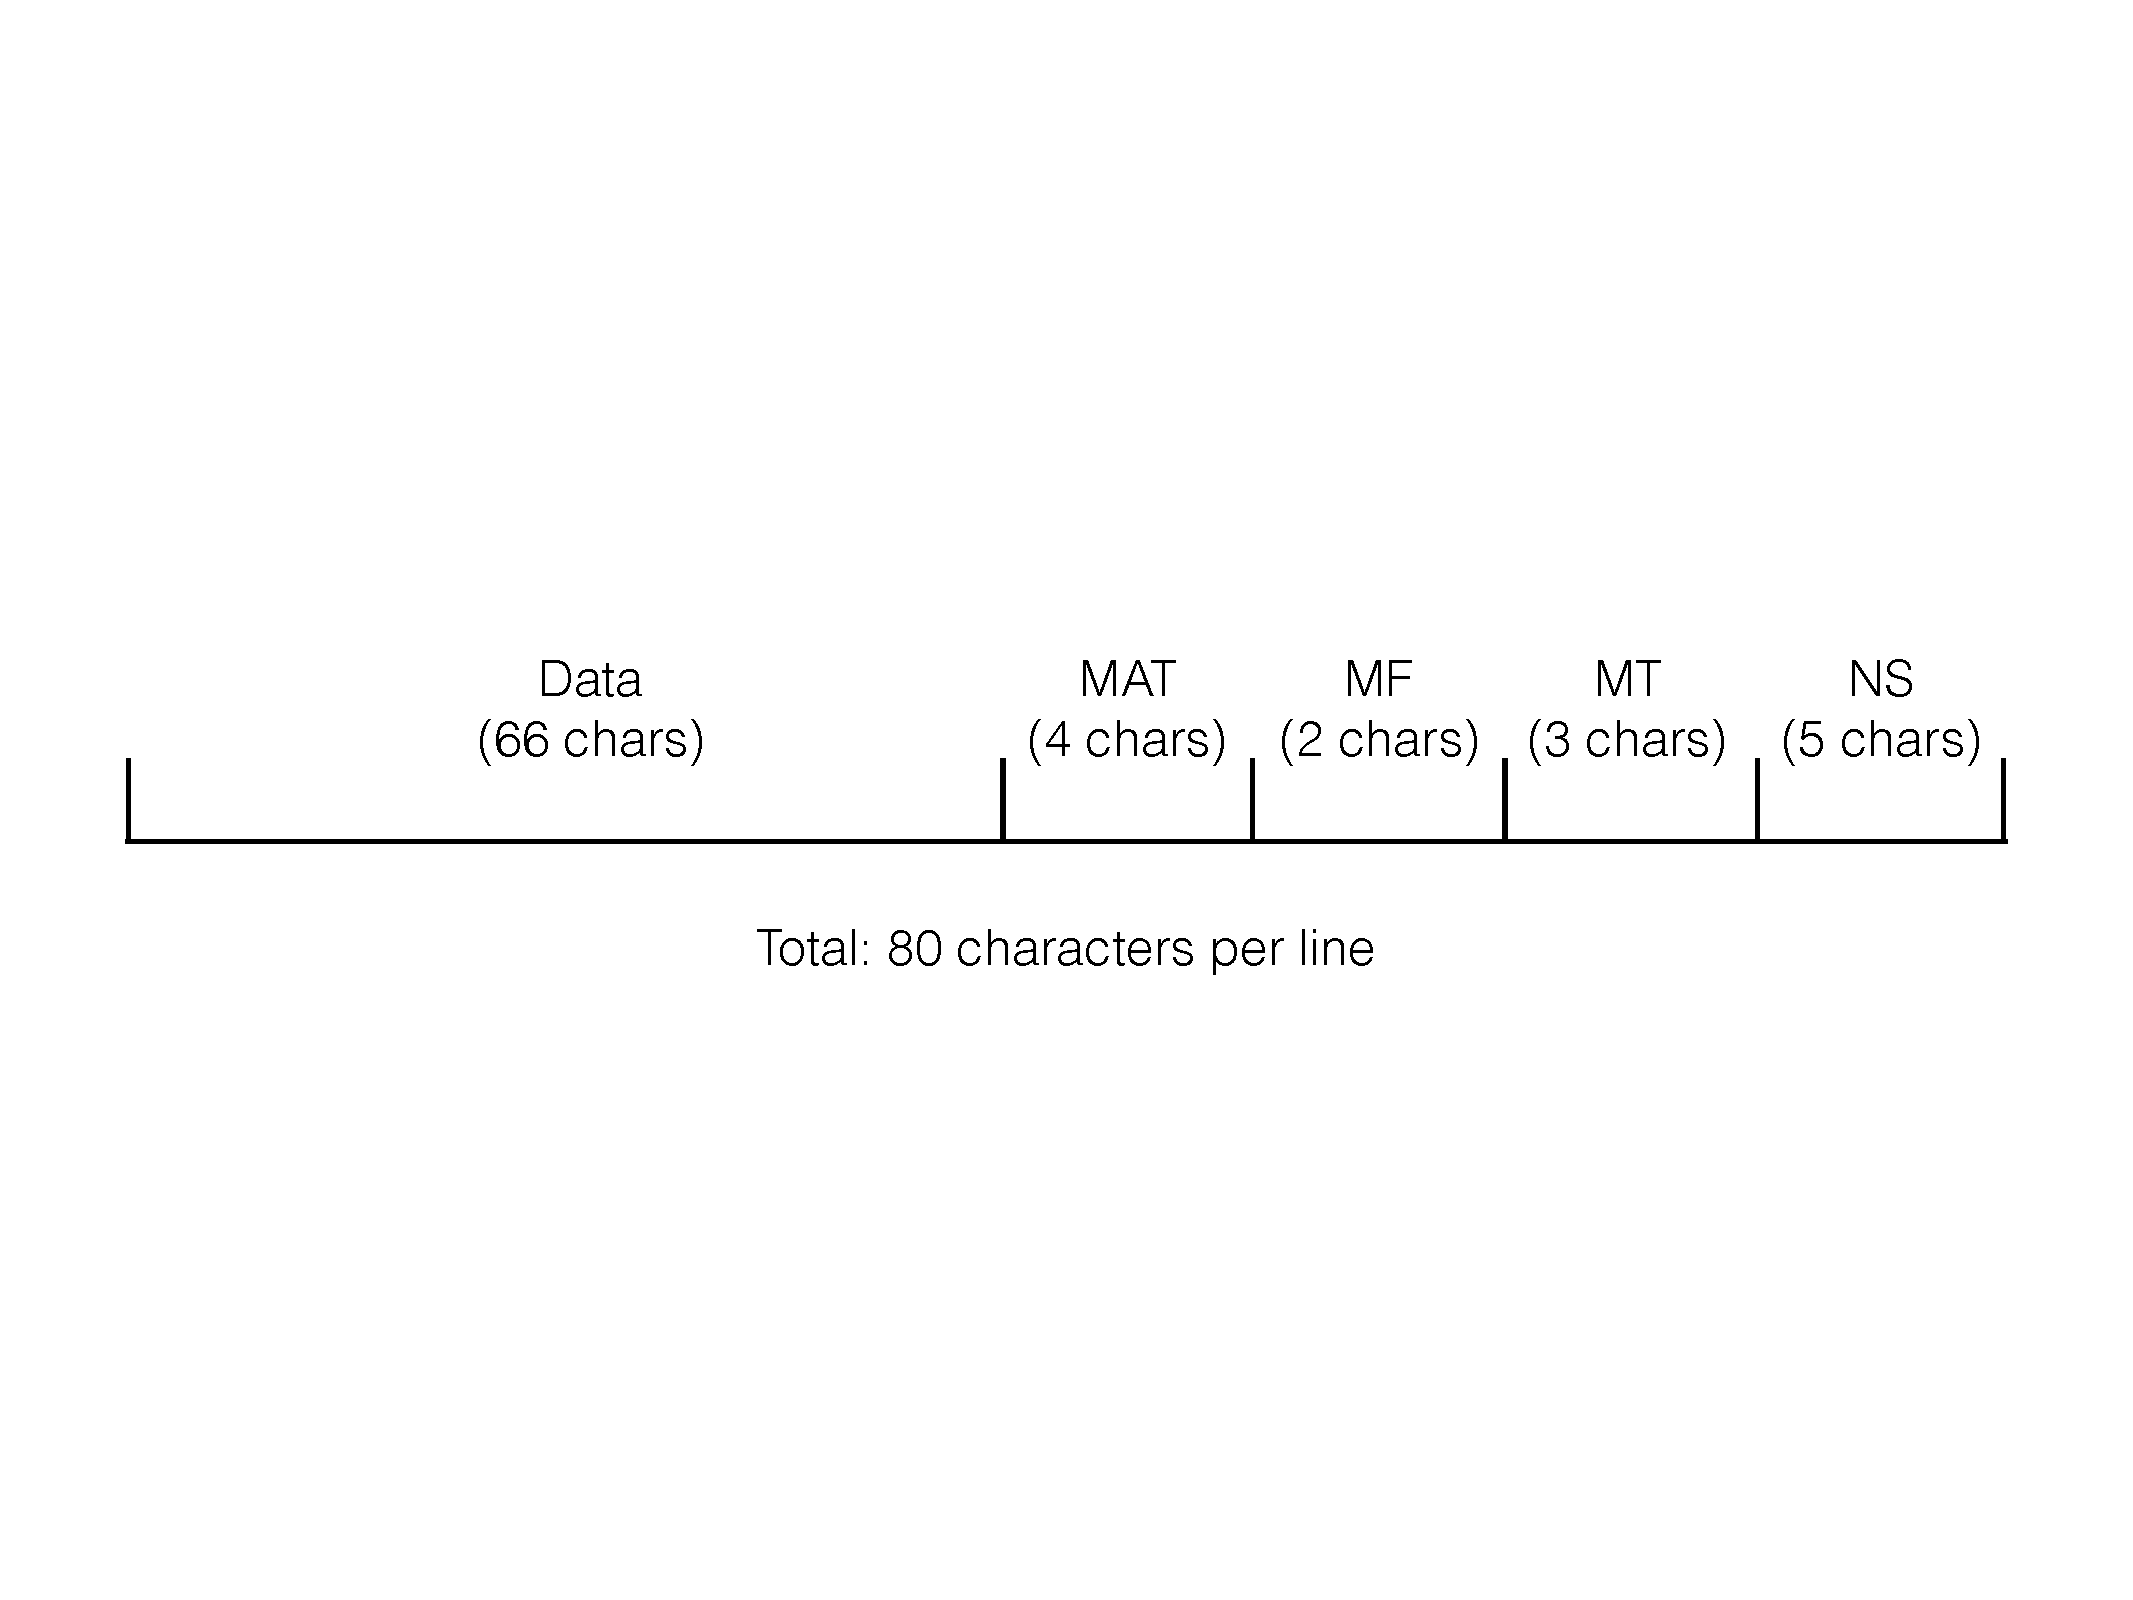
\includegraphics[scale=0.4]{./pics/endf-6-record.pdf}
\end{center}
\caption{ \label{fig:endf-6-record}
An example line of record for ENDF file}
\end{figure}

The ENDF-6 format specifies five types of commonly used records: TEXT, CONT, LIST, TAB1, and TAB2. 

\subsection{TEXT Records}
A TEXT records describes some text information, for example the meta information of the cross section.. The data section of the TEXT record is contains only one field: HL, which takes 66 characters. An illustration of the text record is shown in Figure \ref{fig:endf-6-record-text}.

\begin{figure}[h]
\begin{center}
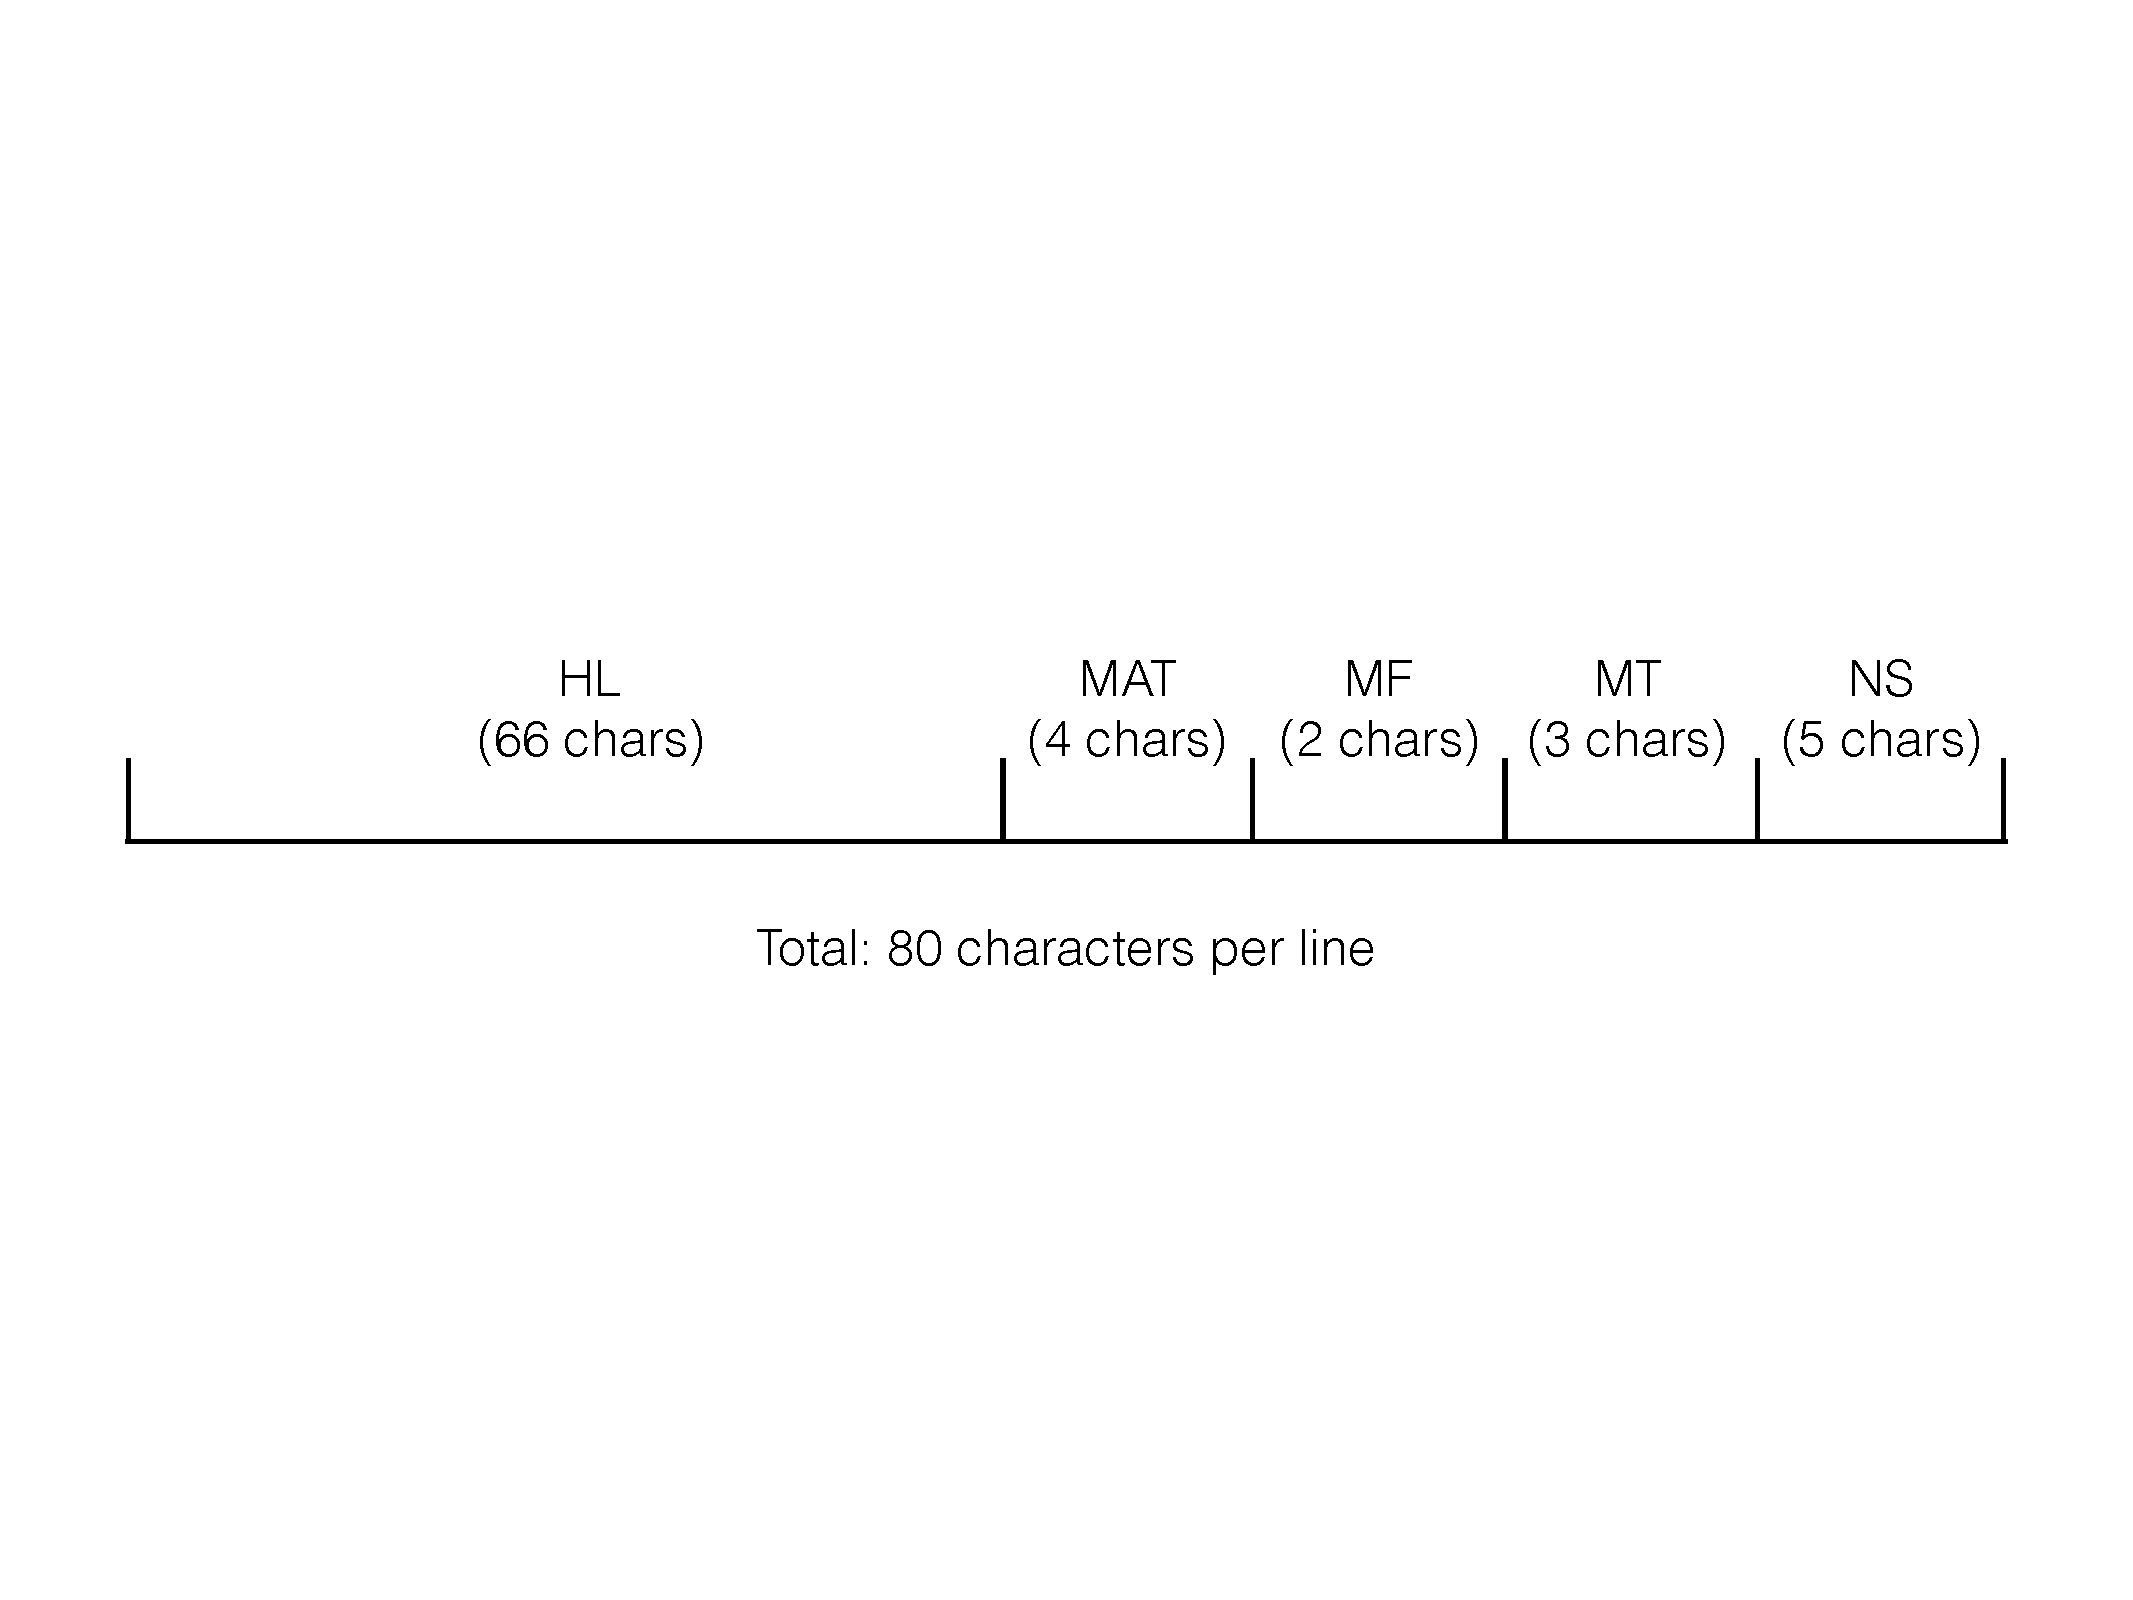
\includegraphics[scale=0.4]{./pics/endf-6-record-text.pdf}
\end{center}
\caption{ \label{fig:endf-6-record-text}
An example line of TEXT record for ENDF file}
\end{figure}

\subsection{CONT Records}
A CONT record includes some control information. The data field contains six floating numbers: C1, C2, L1, L2, N1 and N2. An illustration of the structure is shown in Figure \ref{fig:endf-6-record-cont}.

\begin{figure}[h]
\begin{center}
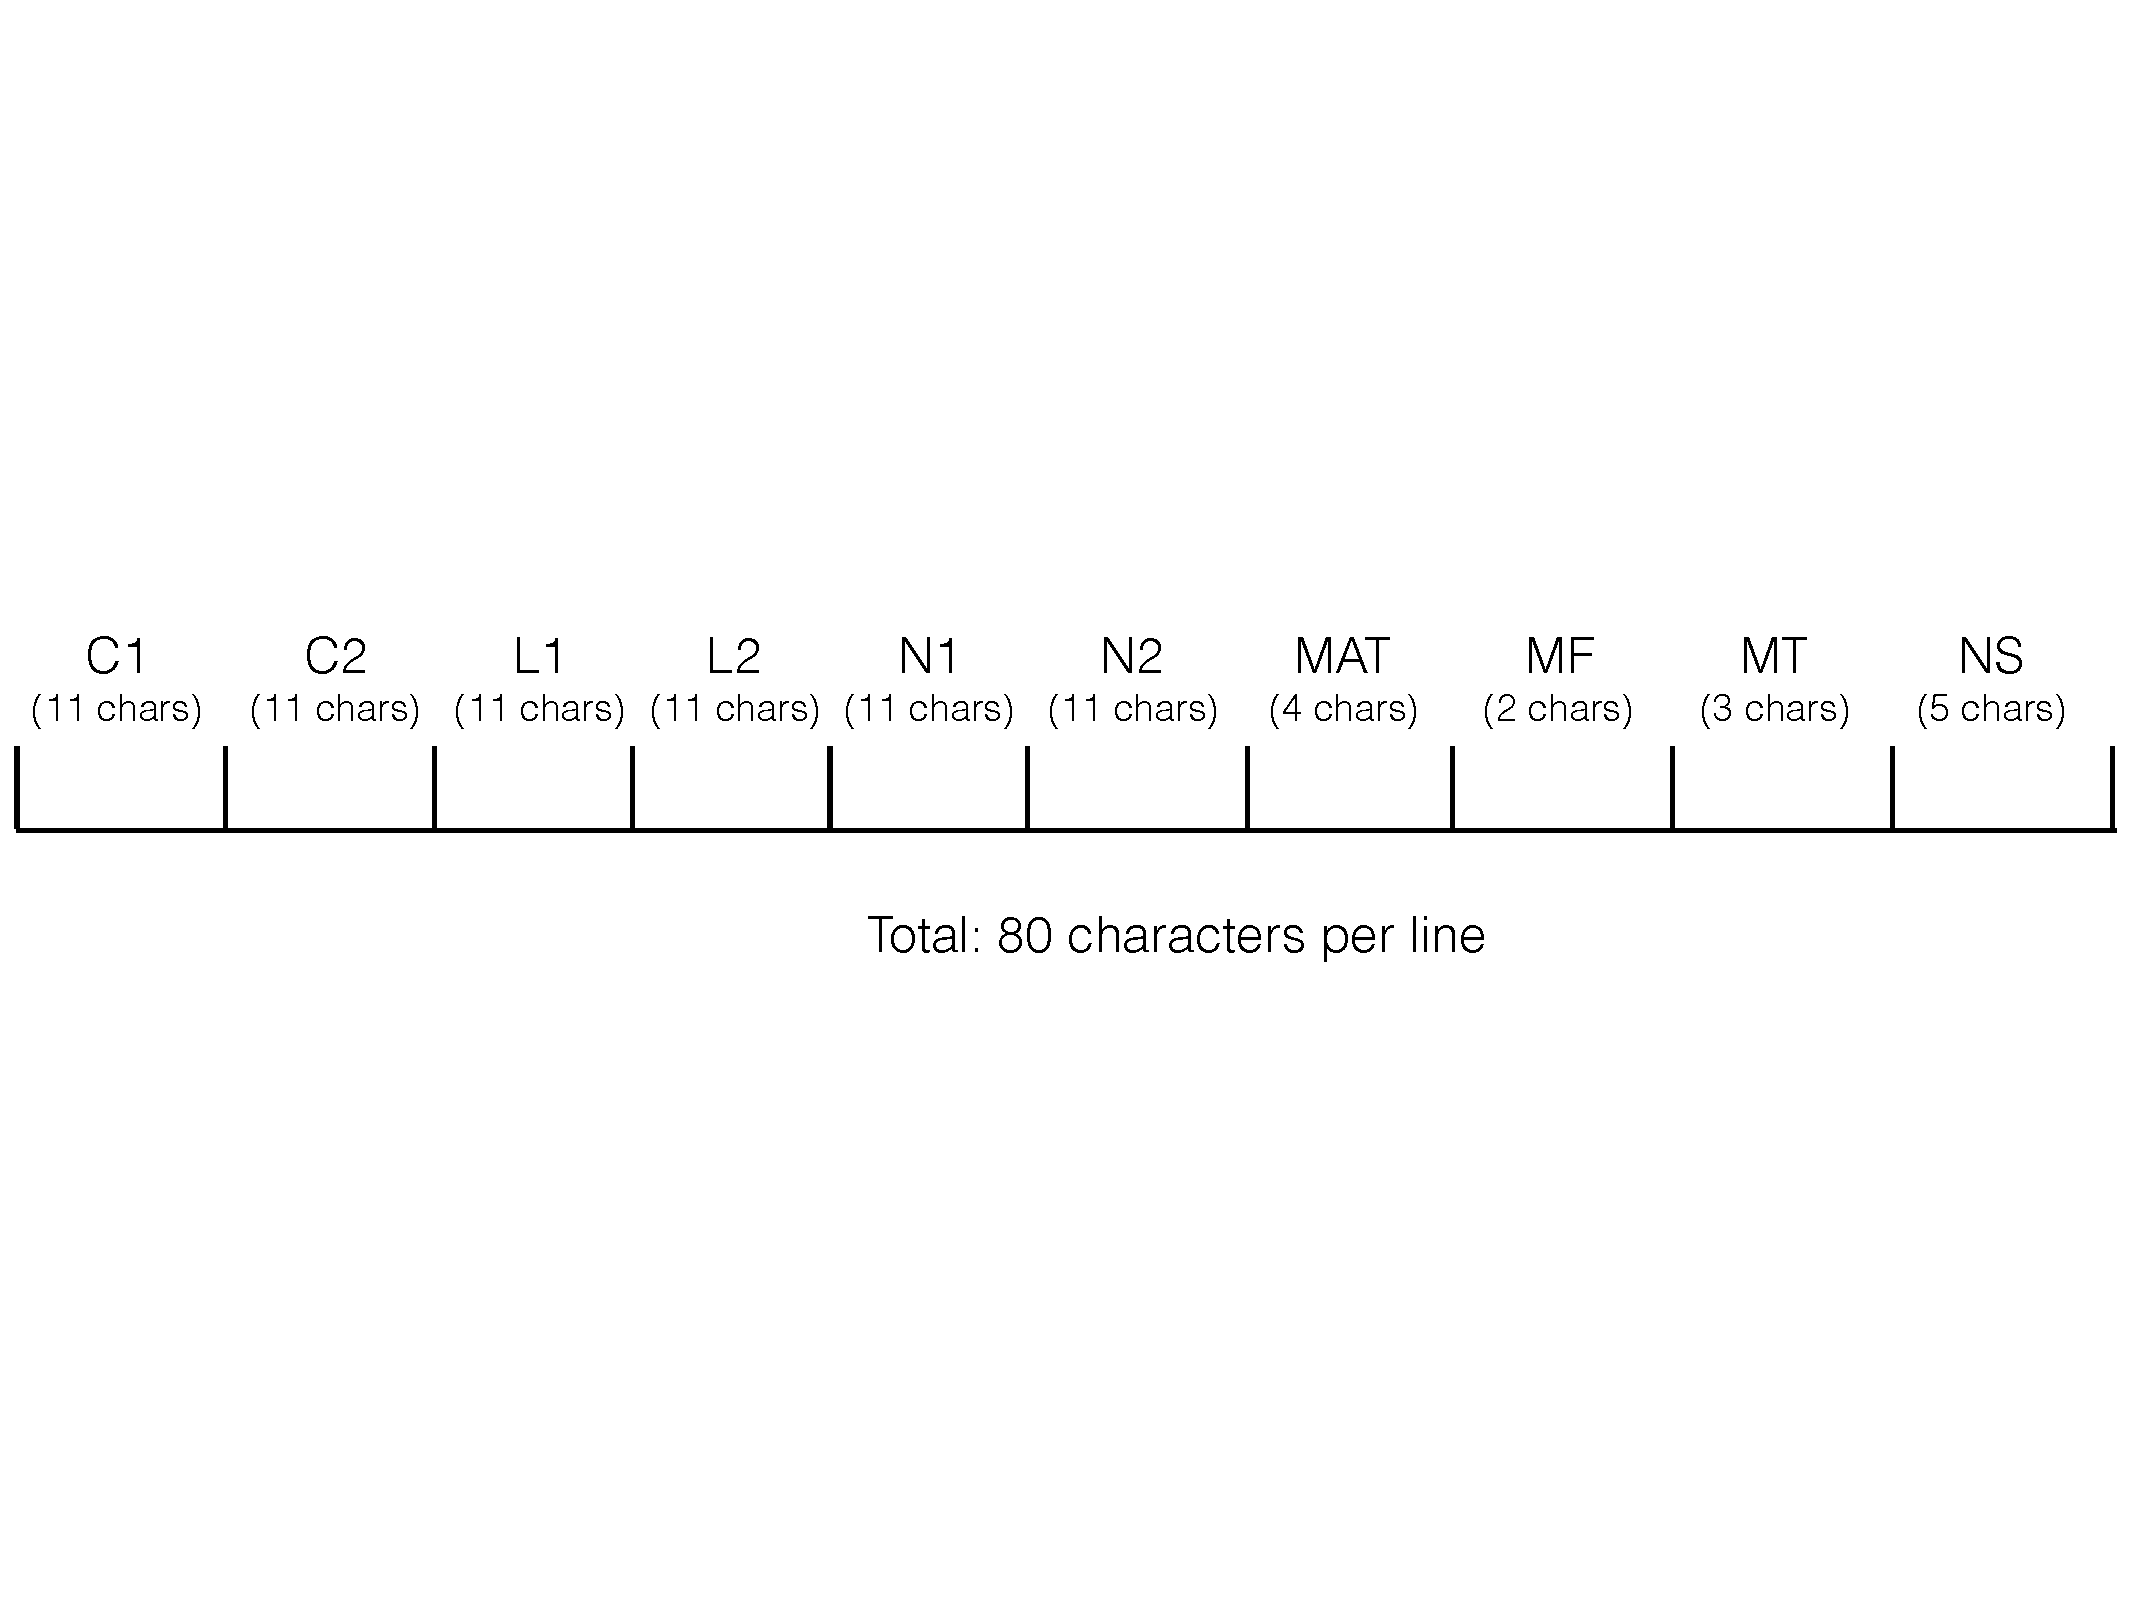
\includegraphics[scale=0.4]{./pics/endf-6-record-cont.pdf}
\end{center}
\caption{ \label{fig:endf-6-record-cont}
An example line of CONT record for ENDF file}
\end{figure}

\subsection{LIST Records}
A LIST record encodes a list of numbers. The records contains multiple lines, where the first line is a CONT record, and followed by a list of numbers organized into packages of 6 numbers. An illustration of these lines are shown in Figure \ref{fig:endf-6-record-list}. The length of list is stored in the 5th argument in the variable NPL in the first line. NPL needs not to be a multiple of 6, since the empty spaces in the list will be filled up with zeros.

\begin{figure}[h]
\begin{center}
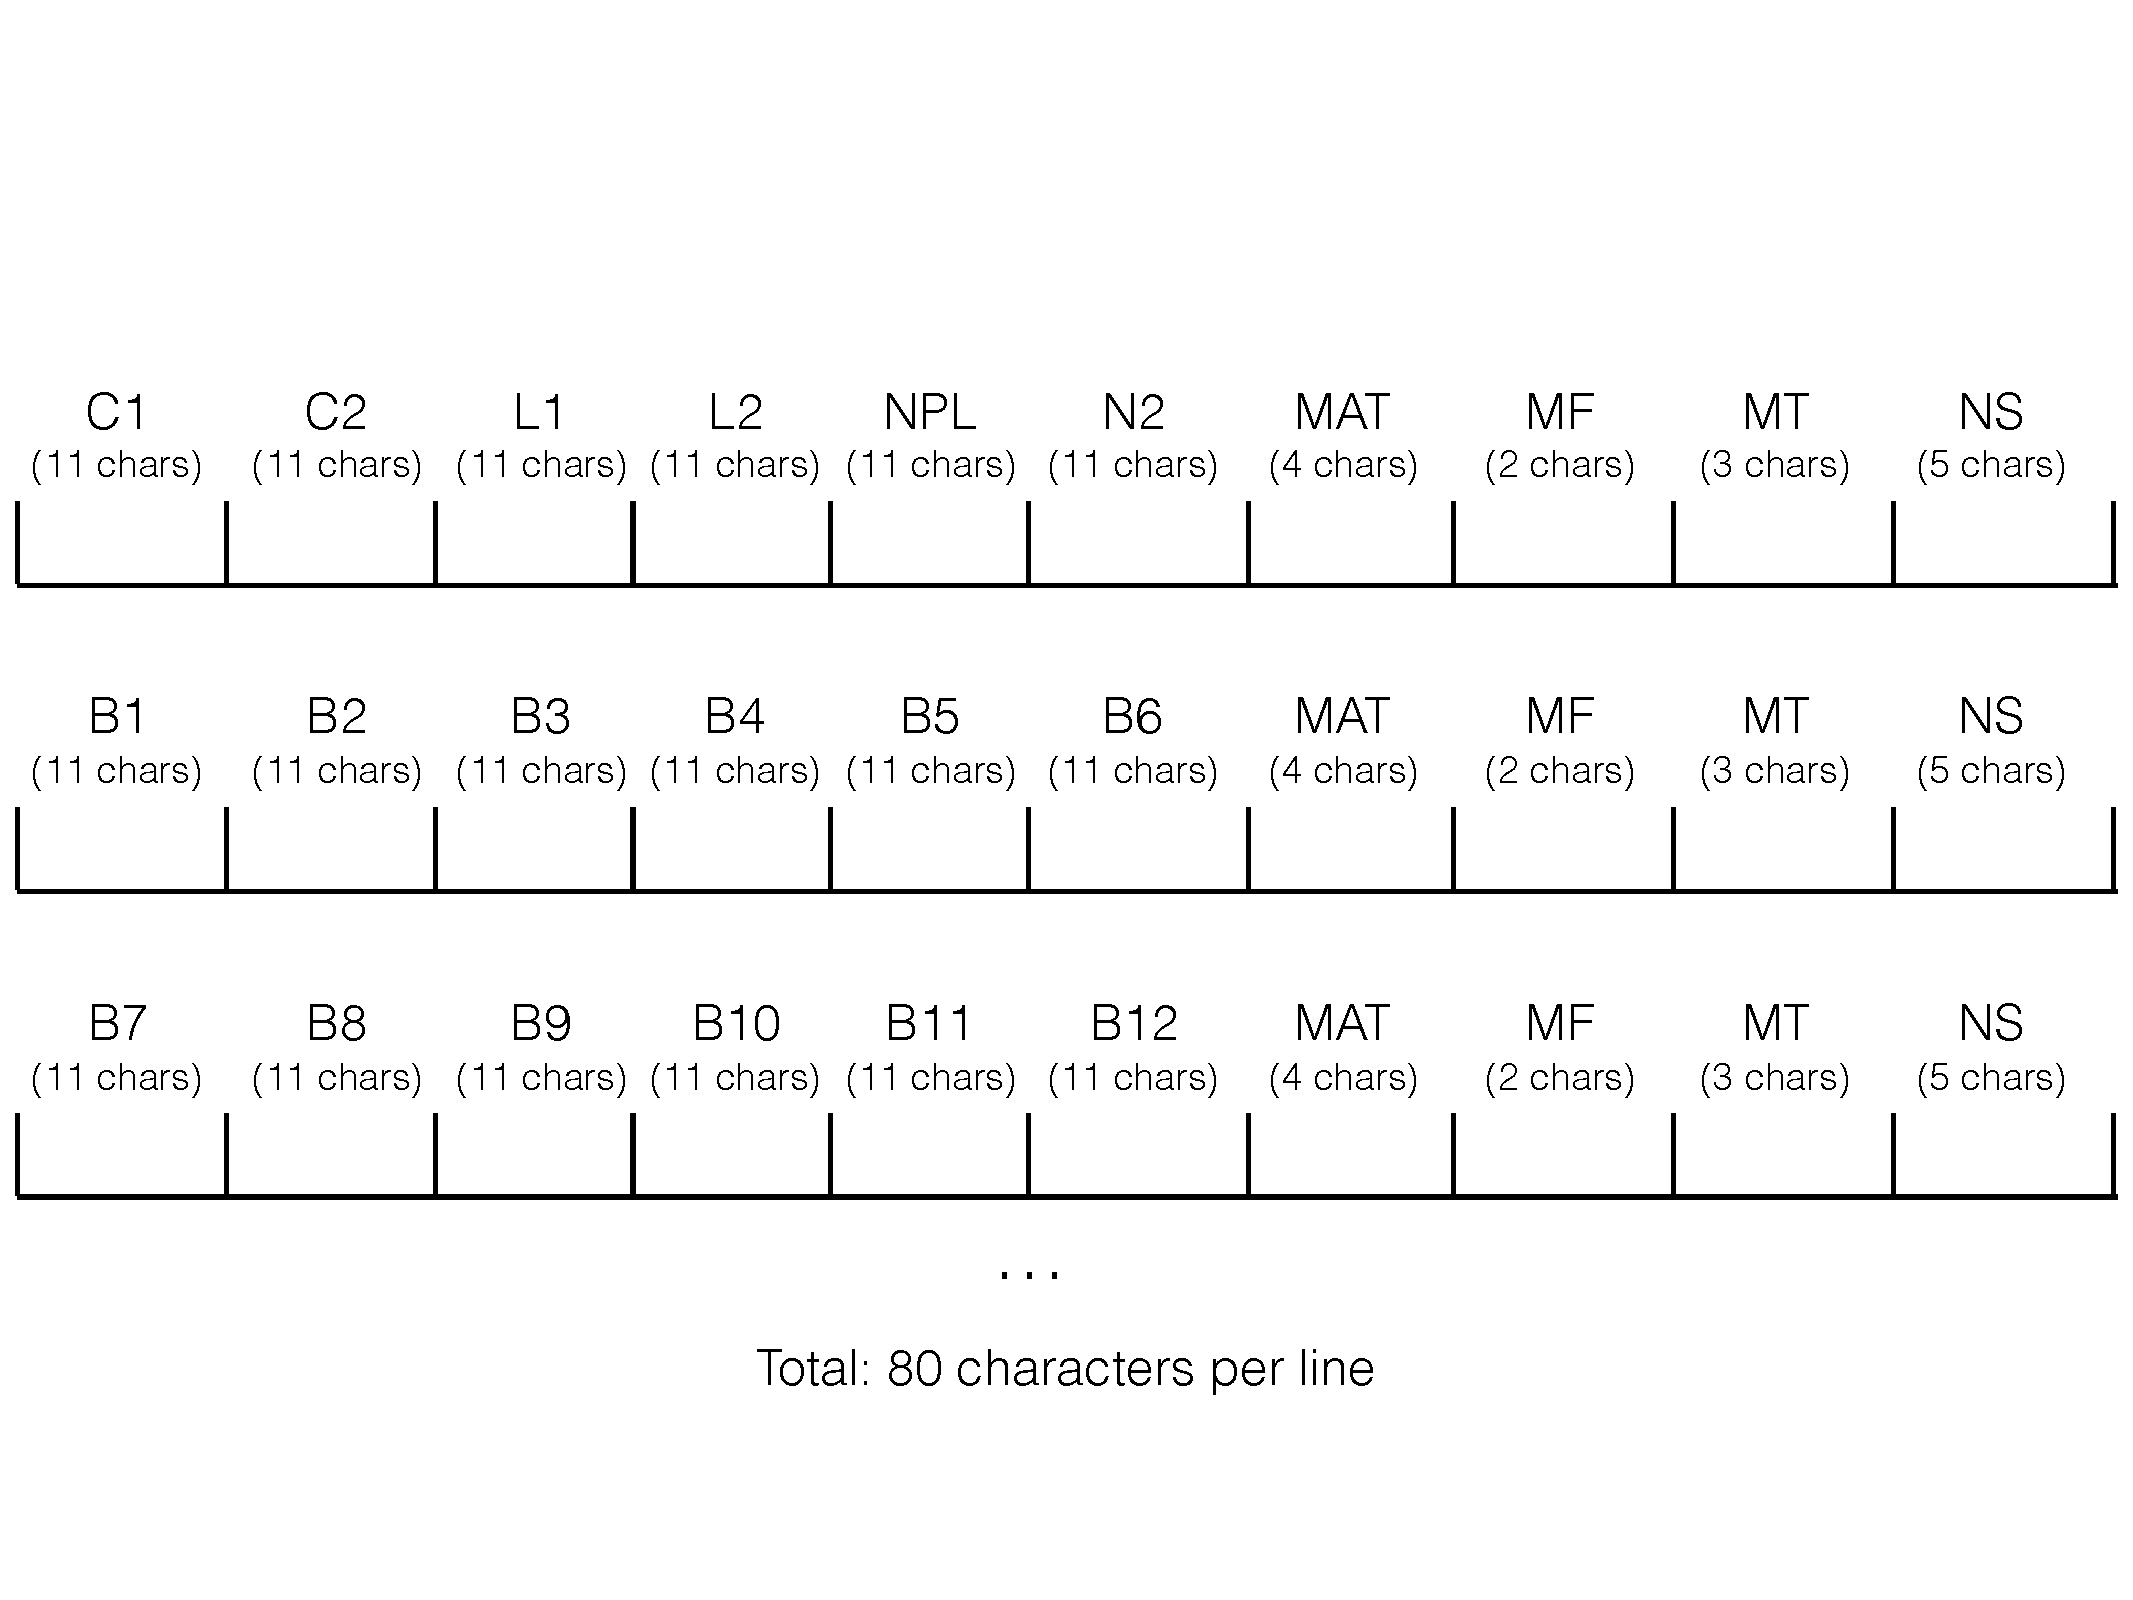
\includegraphics[scale=0.4]{./pics/endf-6-record-list.pdf}
\end{center}
\caption{ \label{fig:endf-6-record-list}
An example line of LIST record for ENDF file}
\end{figure}

\subsection{TAB1 Records}
A TAB1 record contains a one-dimensional tabulated functions such as $y(x)$. To describe the table function, four lists of data are presenting: NBT, INT, X, and Y. The dimensions of NBT and INT are NR, and the dimensions of X and Y are NP. This section of data contains a control record at the beginning, then followed by pairs of (NBT, INT) and pairs of (X, Y). An illustration of the storage format is shown in Figure \ref{fig:endf-6-record-tab1}.

\begin{figure}[h]
\begin{center}
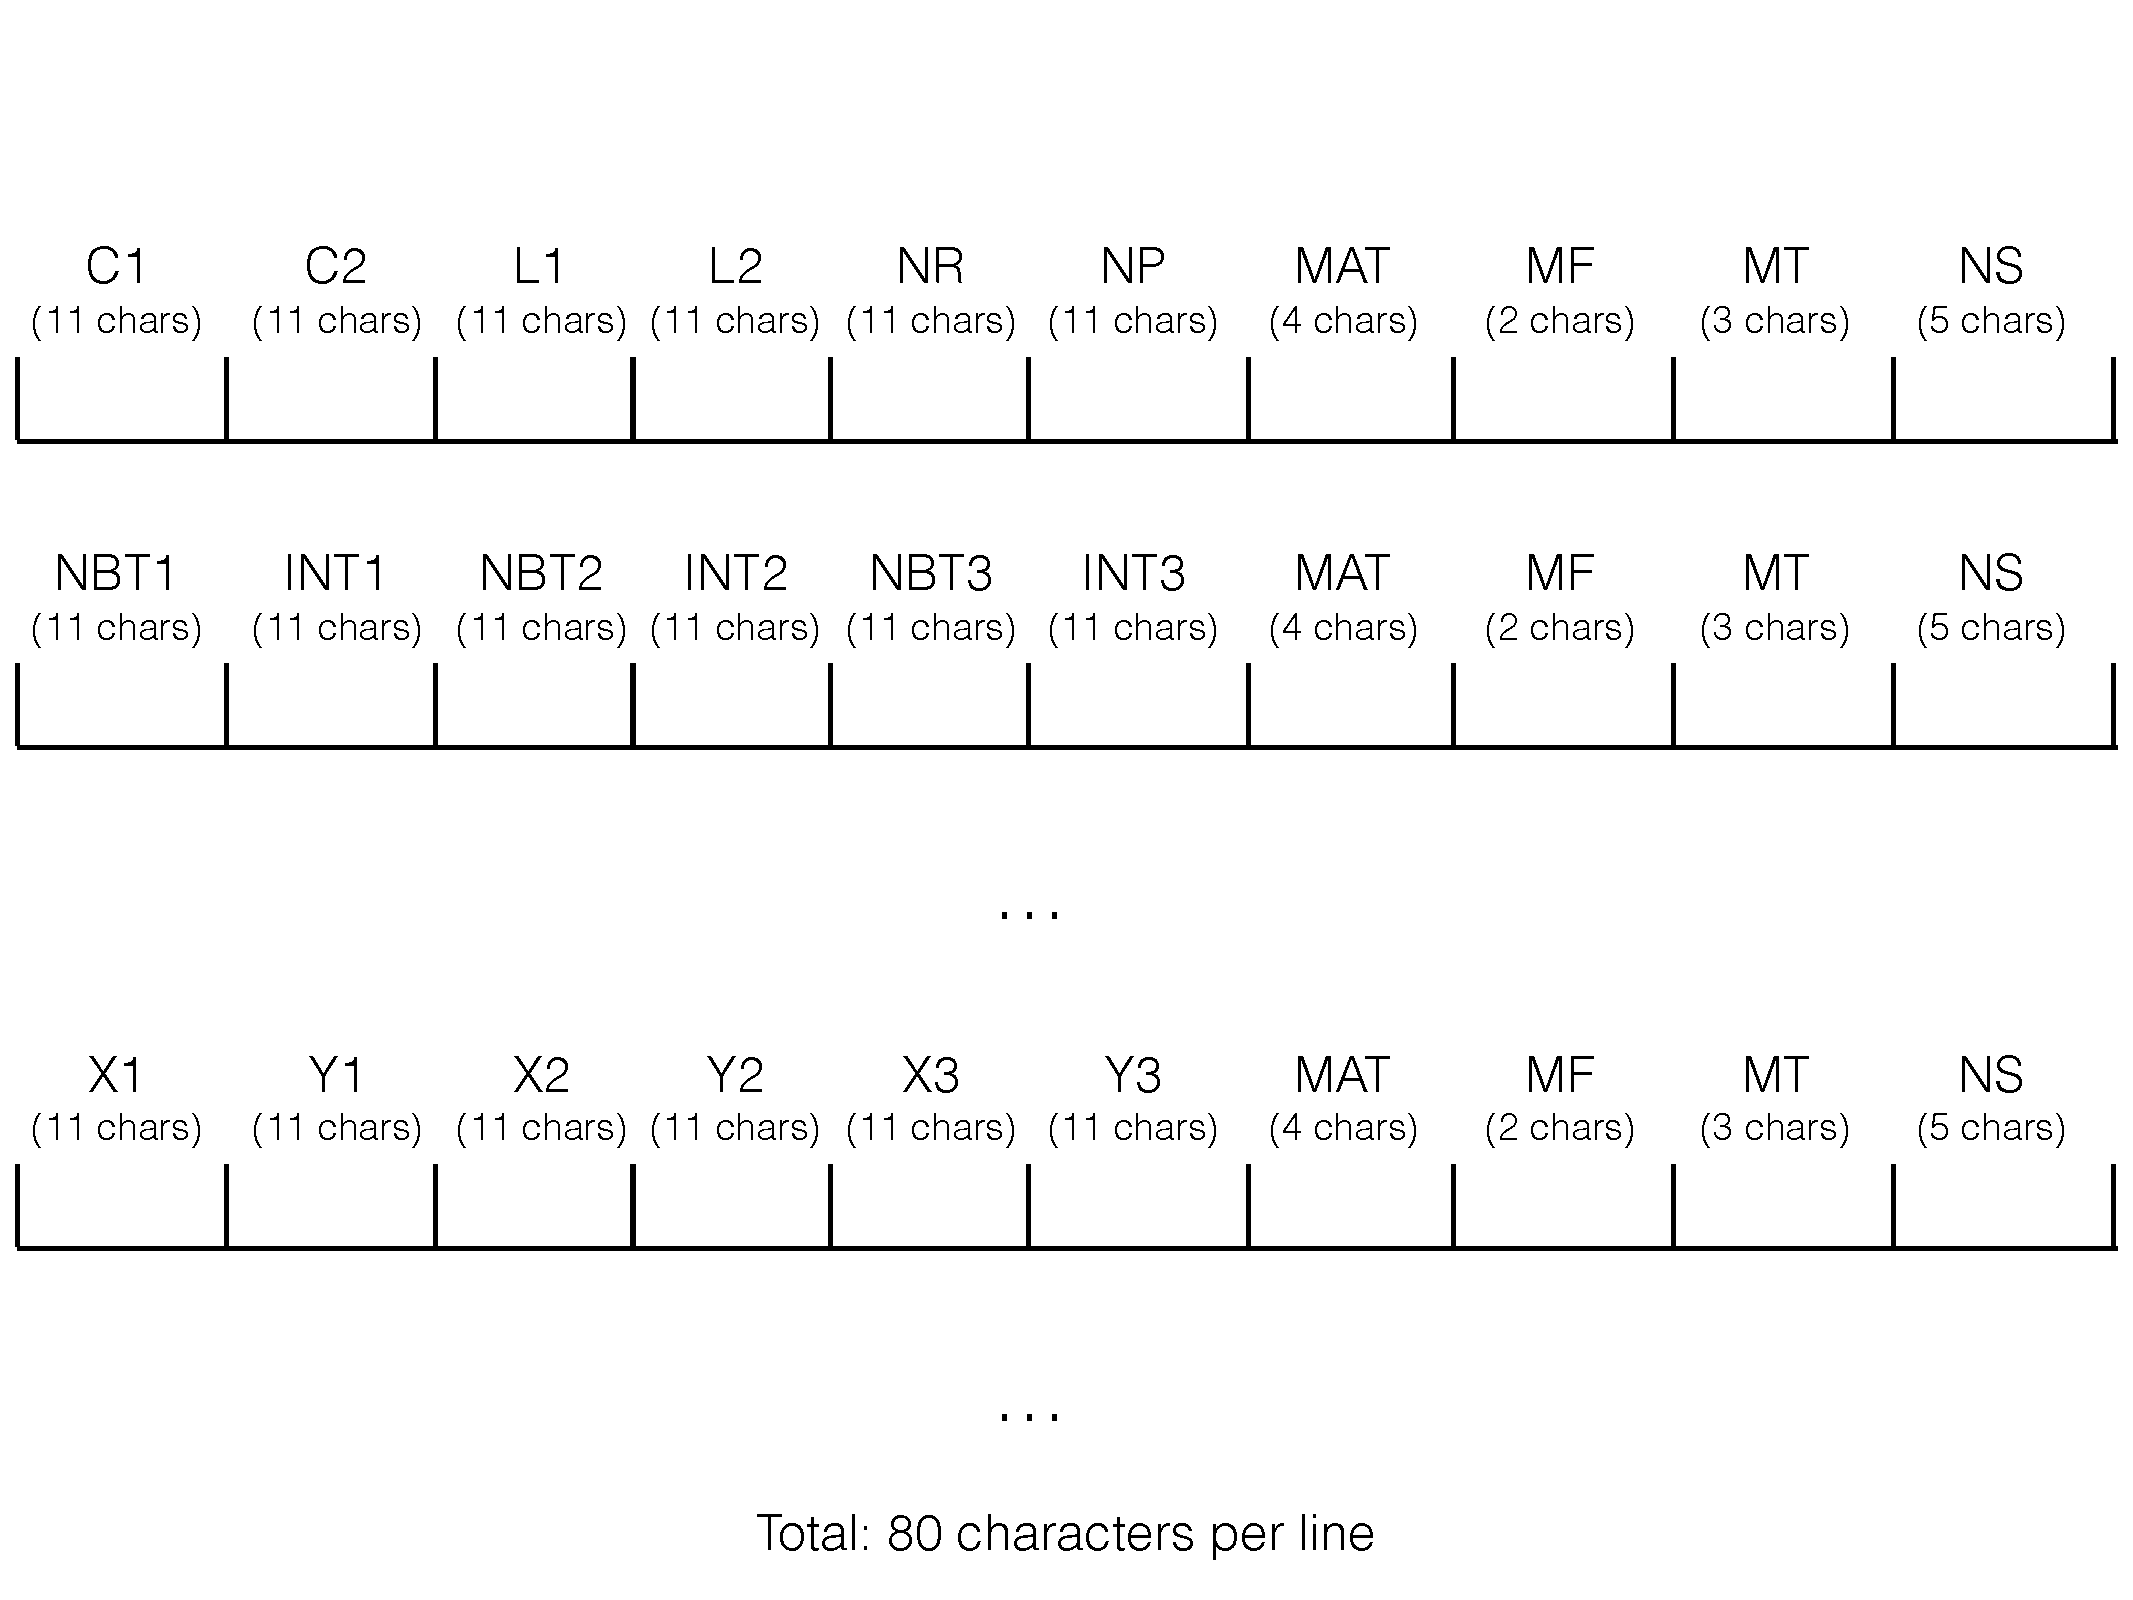
\includegraphics[scale=0.4]{./pics/endf-6-record-tab1.pdf}
\end{center}
\caption{ \label{fig:endf-6-record-tab1}
An example line of TAB1 record for ENDF file}
\end{figure}

\subsection{TAB2 Records}
A TAB2 record contains a two-dimensional tabular functions such as $y(x,z)$. The TAB2 records storages a list of data points for the $z$ variable and the interpolation rules in the NBT and INT array. It follows by NZ records with the C2 designated for the corresponding $z$ value. The possible records followed are either TAB1 or LIST record. An illustration of the format of storage is shown in Figure \ref{fig:endf-6-record-tab2}.

\begin{figure}[h]
\begin{center}
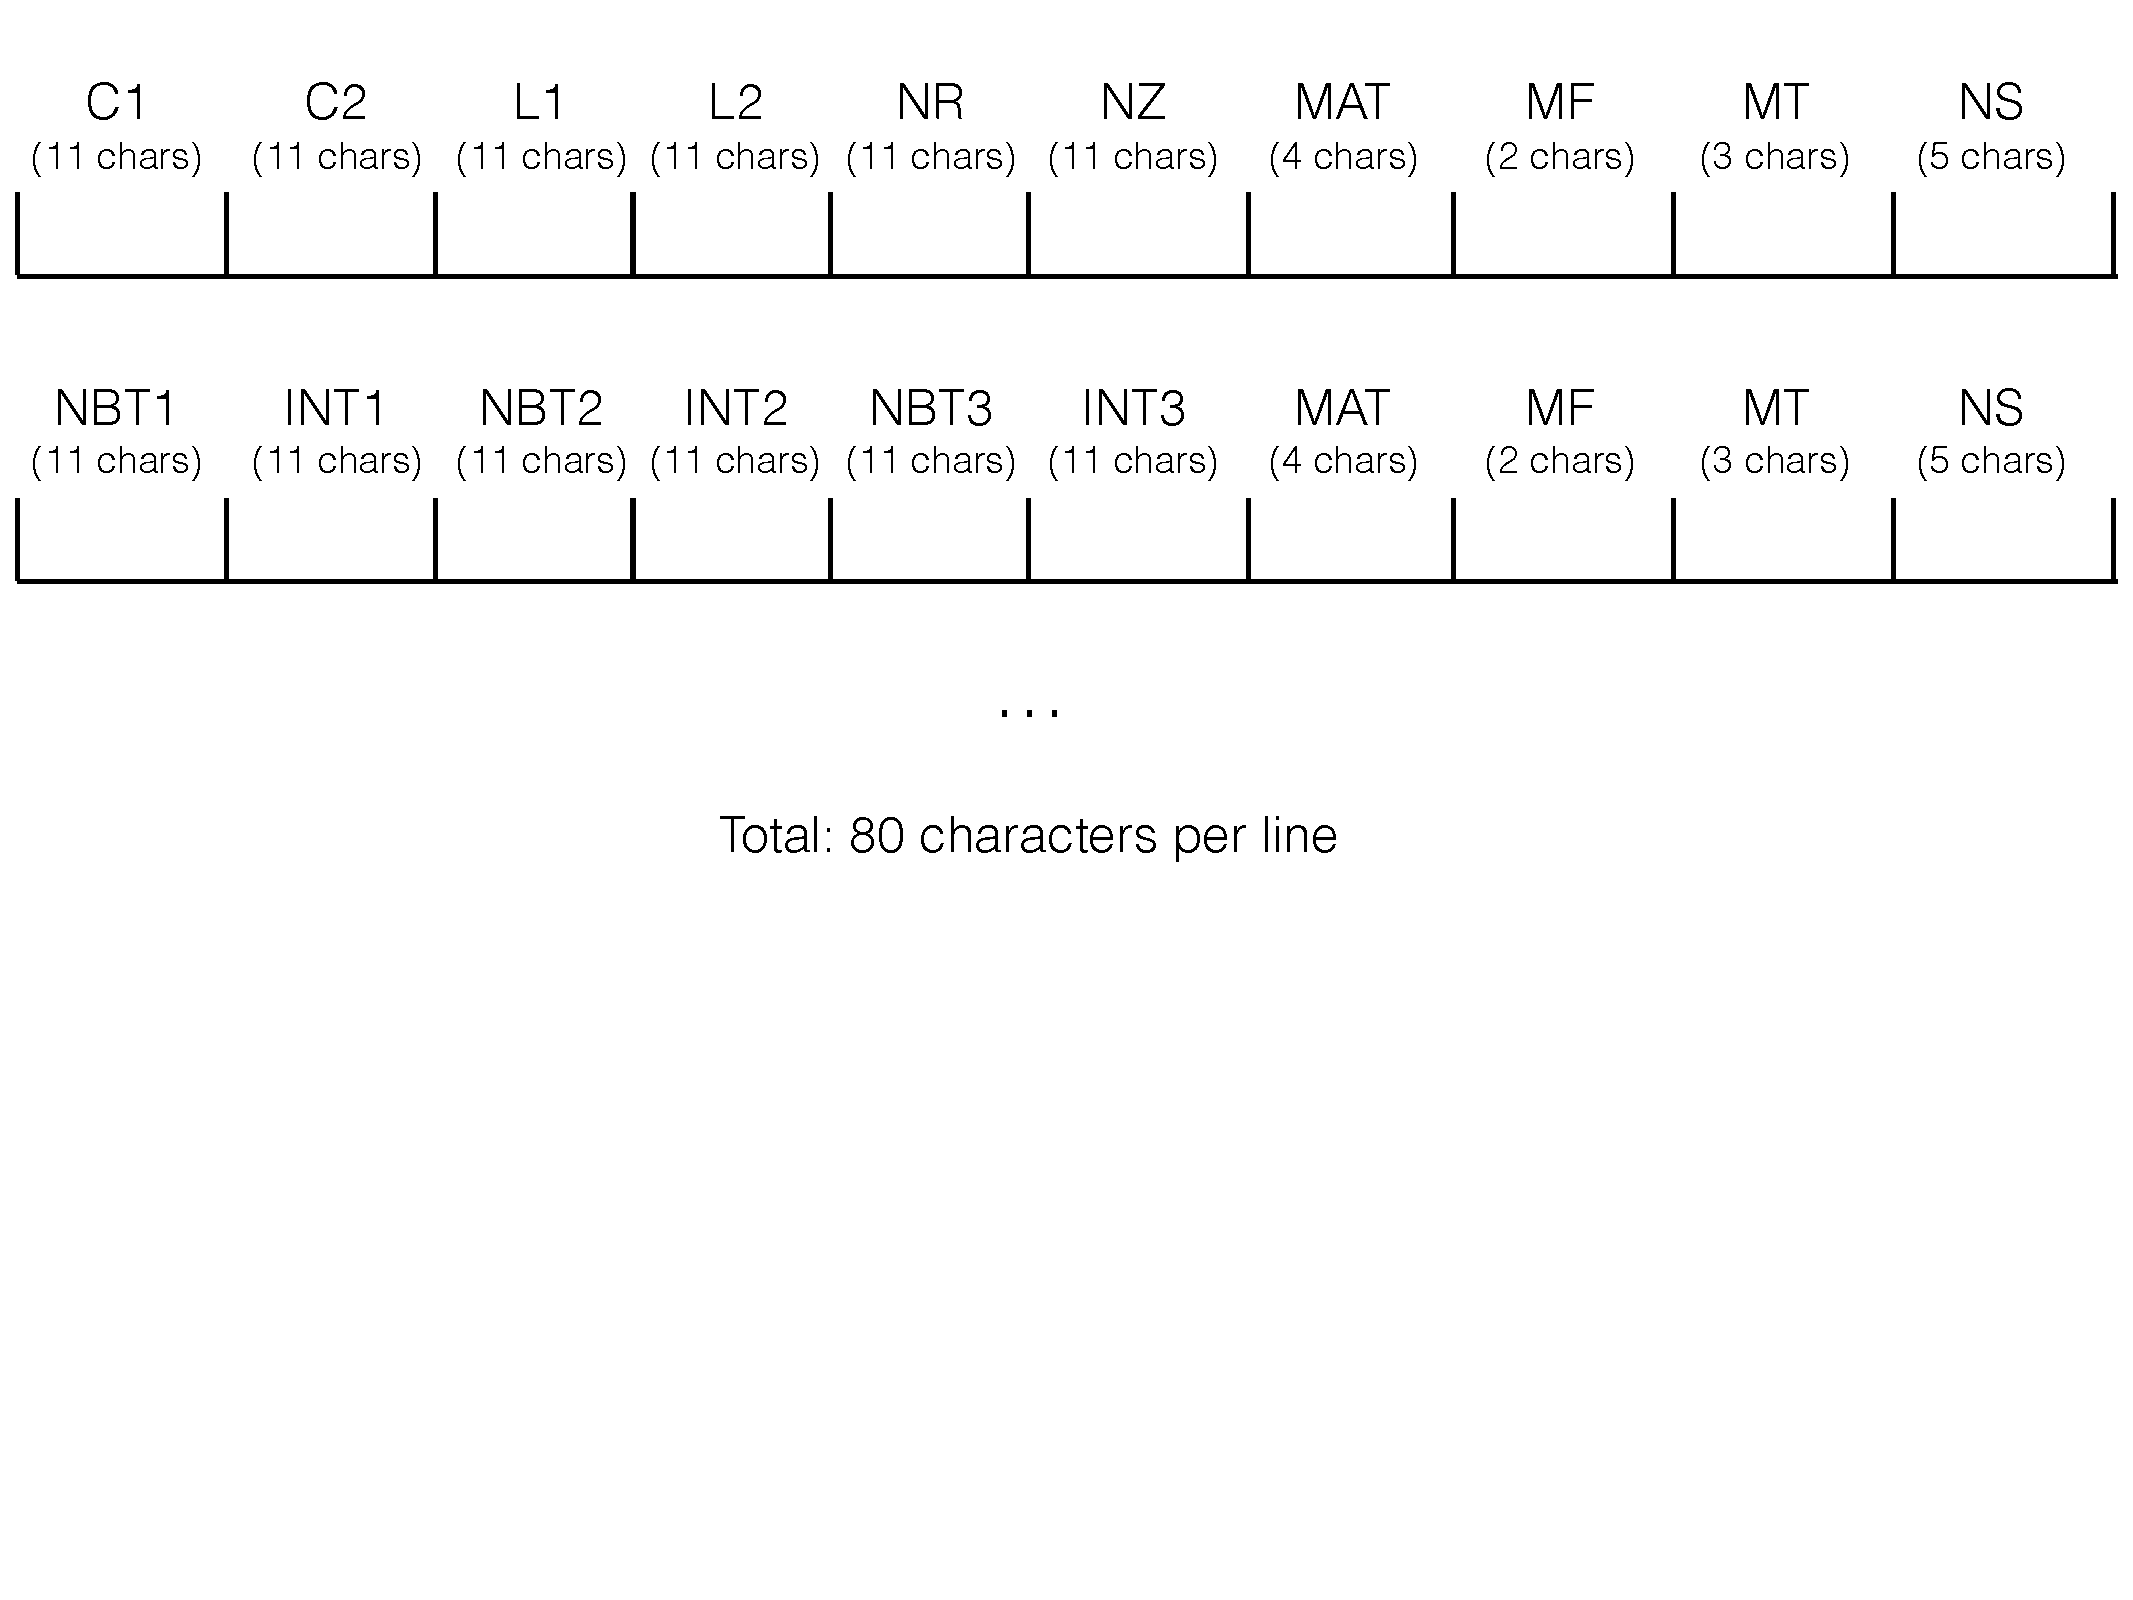
\includegraphics[scale=0.4]{./pics/endf-6-record-tab2.pdf}
\end{center}
\caption{ \label{fig:endf-6-record-tab2}
An example line of TAB2 record for ENDF file}
\end{figure}

\clearpage
\section{C++ Data Structure \& Application Interfaces}
The program is implemented native in C++ programming language, so in this section, we discuss the data structures first then the application interfaces.

The top level neutron data structure contains several major parts: the fission yield data, the reaction data, and the resonance data, as followed. 
\begin{verbatim} 
struct ENDFNeutronData {

    ... definitions of support data structures ...

    /* Key data structures for neutron data */
    
    // The fission yield information, from File 1 and 5
    YieldData                  fissionYield;
    
    // List of reactions information, from File 3
    std::vector<ReactionData>  reactions;
    
    // List of resonances information, from File 2
    std::vector<ResonanceData> resonances;
}
\end{verbatim}
The discussion begins with lower level data structures, and then discuss each major part in details.

\subsection{Fundamental Computational Data Structures}

\begin{itemize}
\item{\em Interpolation function: } 
The law of interpolation is a structure contains two fields: INT for the interpolation form, and NBT for the interpolation index.
\begin{verbatim} 
struct ENDFInterpLaw {
    long INT = -1;
    long NBT = -1;
};
\end{verbatim}
The law of interpolation is used in a list, i.e. 
\begin{verbatim} 
std::vector<ENDFInterpLaw> 
\end{verbatim}
, which is usually combined with a list of scattered function values with $x-y$ pairs. One such pair is called a datapoint, which is defined in a structure as followed:
\begin{verbatim} 
template <typename T>
struct ENDFObjectDataPoint {
    double x = 0.;
    T y;
};
\end{verbatim}
$x$ value is a scalar of floating number, and the $y$ value can be any object, and is expressed in a C++ template class parameter. A special case where $y$ is a scalar floating number as well is defined as a special type ENDFDataPoint.
\begin{verbatim} 
typedef ENDFObjectDataPoint<double>   ENDFDataPoint;
\end{verbatim}
A tabular function is represented by a list of ENDFInterpLaw and a list of ENDFDataPoint:
\begin{verbatim}
struct ENDFInterpolationFunction {
    std::vector< ENDFInterpLaw > interp;
    std::vector< ENDFDataPoint > data;
    
    // Evaluate the interpolation function at point x
    double evaluate(double x) const;
};
\end{verbatim}
The meaning of the integer INT is listed in table \ref{tab:interp}.
\begin{table}[h]
\centering
\caption{Definition of interpolation laws}
\vspace{1ex}
\begin{tabular}{L{2cm} L{6cm}}
\hline 
INT & Interpolation Scheme \\
\hline
1 & $y$ is constant in $x$ \\
2 & $y$ is linear in $x$\\
3 & $y$ is linear in $\ln(x)$ \\
4 & $\ln(y)$ is linear in $x$ \\
5 & $\ln(y)$ is linear in $\ln(x)$\\
\hline
\end{tabular}
\label{tab:interp}
\end{table}
Next, we illustrate how to interpolate the function at any given $x$ with an example, as shown in Figure \ref{fig:endf-int-laws}, taken from the ENDF manual. In this function, we have 10 data points which splits into 3 regions, the NBT numbers are marked to indicate the upper boundaries of the regions. The INT numbers indicate the interpolation laws of the regions, as explained in Table \ref{tab:interp}. It is possible that two points share the same $x$-coordinate, and this point relates to a `jump' in the function. For a given $x$ between two points $(x_l, y_l)$ and $(x_r, y_r)$ with an interpolation law INT. Then, the interpolated $y$ is calculated by:
\begin{eqnarray}
y &=& y_l, \mbox{ if INT} = 1,\\[1ex]
y &=& y_l + \frac{x-x_l}{x_r-x_l}(y_r-y_l),  \mbox{ if INT} = 2,\\[1ex]
y &=& y_l + \frac{\log(x/x_l)}{\log(x_r/x_l)}(y_r-y_l),  \mbox{ if INT} = 3,\\[1ex]
y &=& y_l \left(\frac{y_r}{y_l}\right)^{\left(\frac{x-x_l}{x_r-x_l}\right)},  \mbox{ if INT} = 4,\\[1ex]
y &=& y_l \left(\frac{y_r}{y_l}\right)^{\left(\frac{\log(x/x_l)}{\log(x_r/x_l)}\right)},  \mbox{ if INT} = 5.
\end{eqnarray}

\begin{figure}[h]
\begin{center}
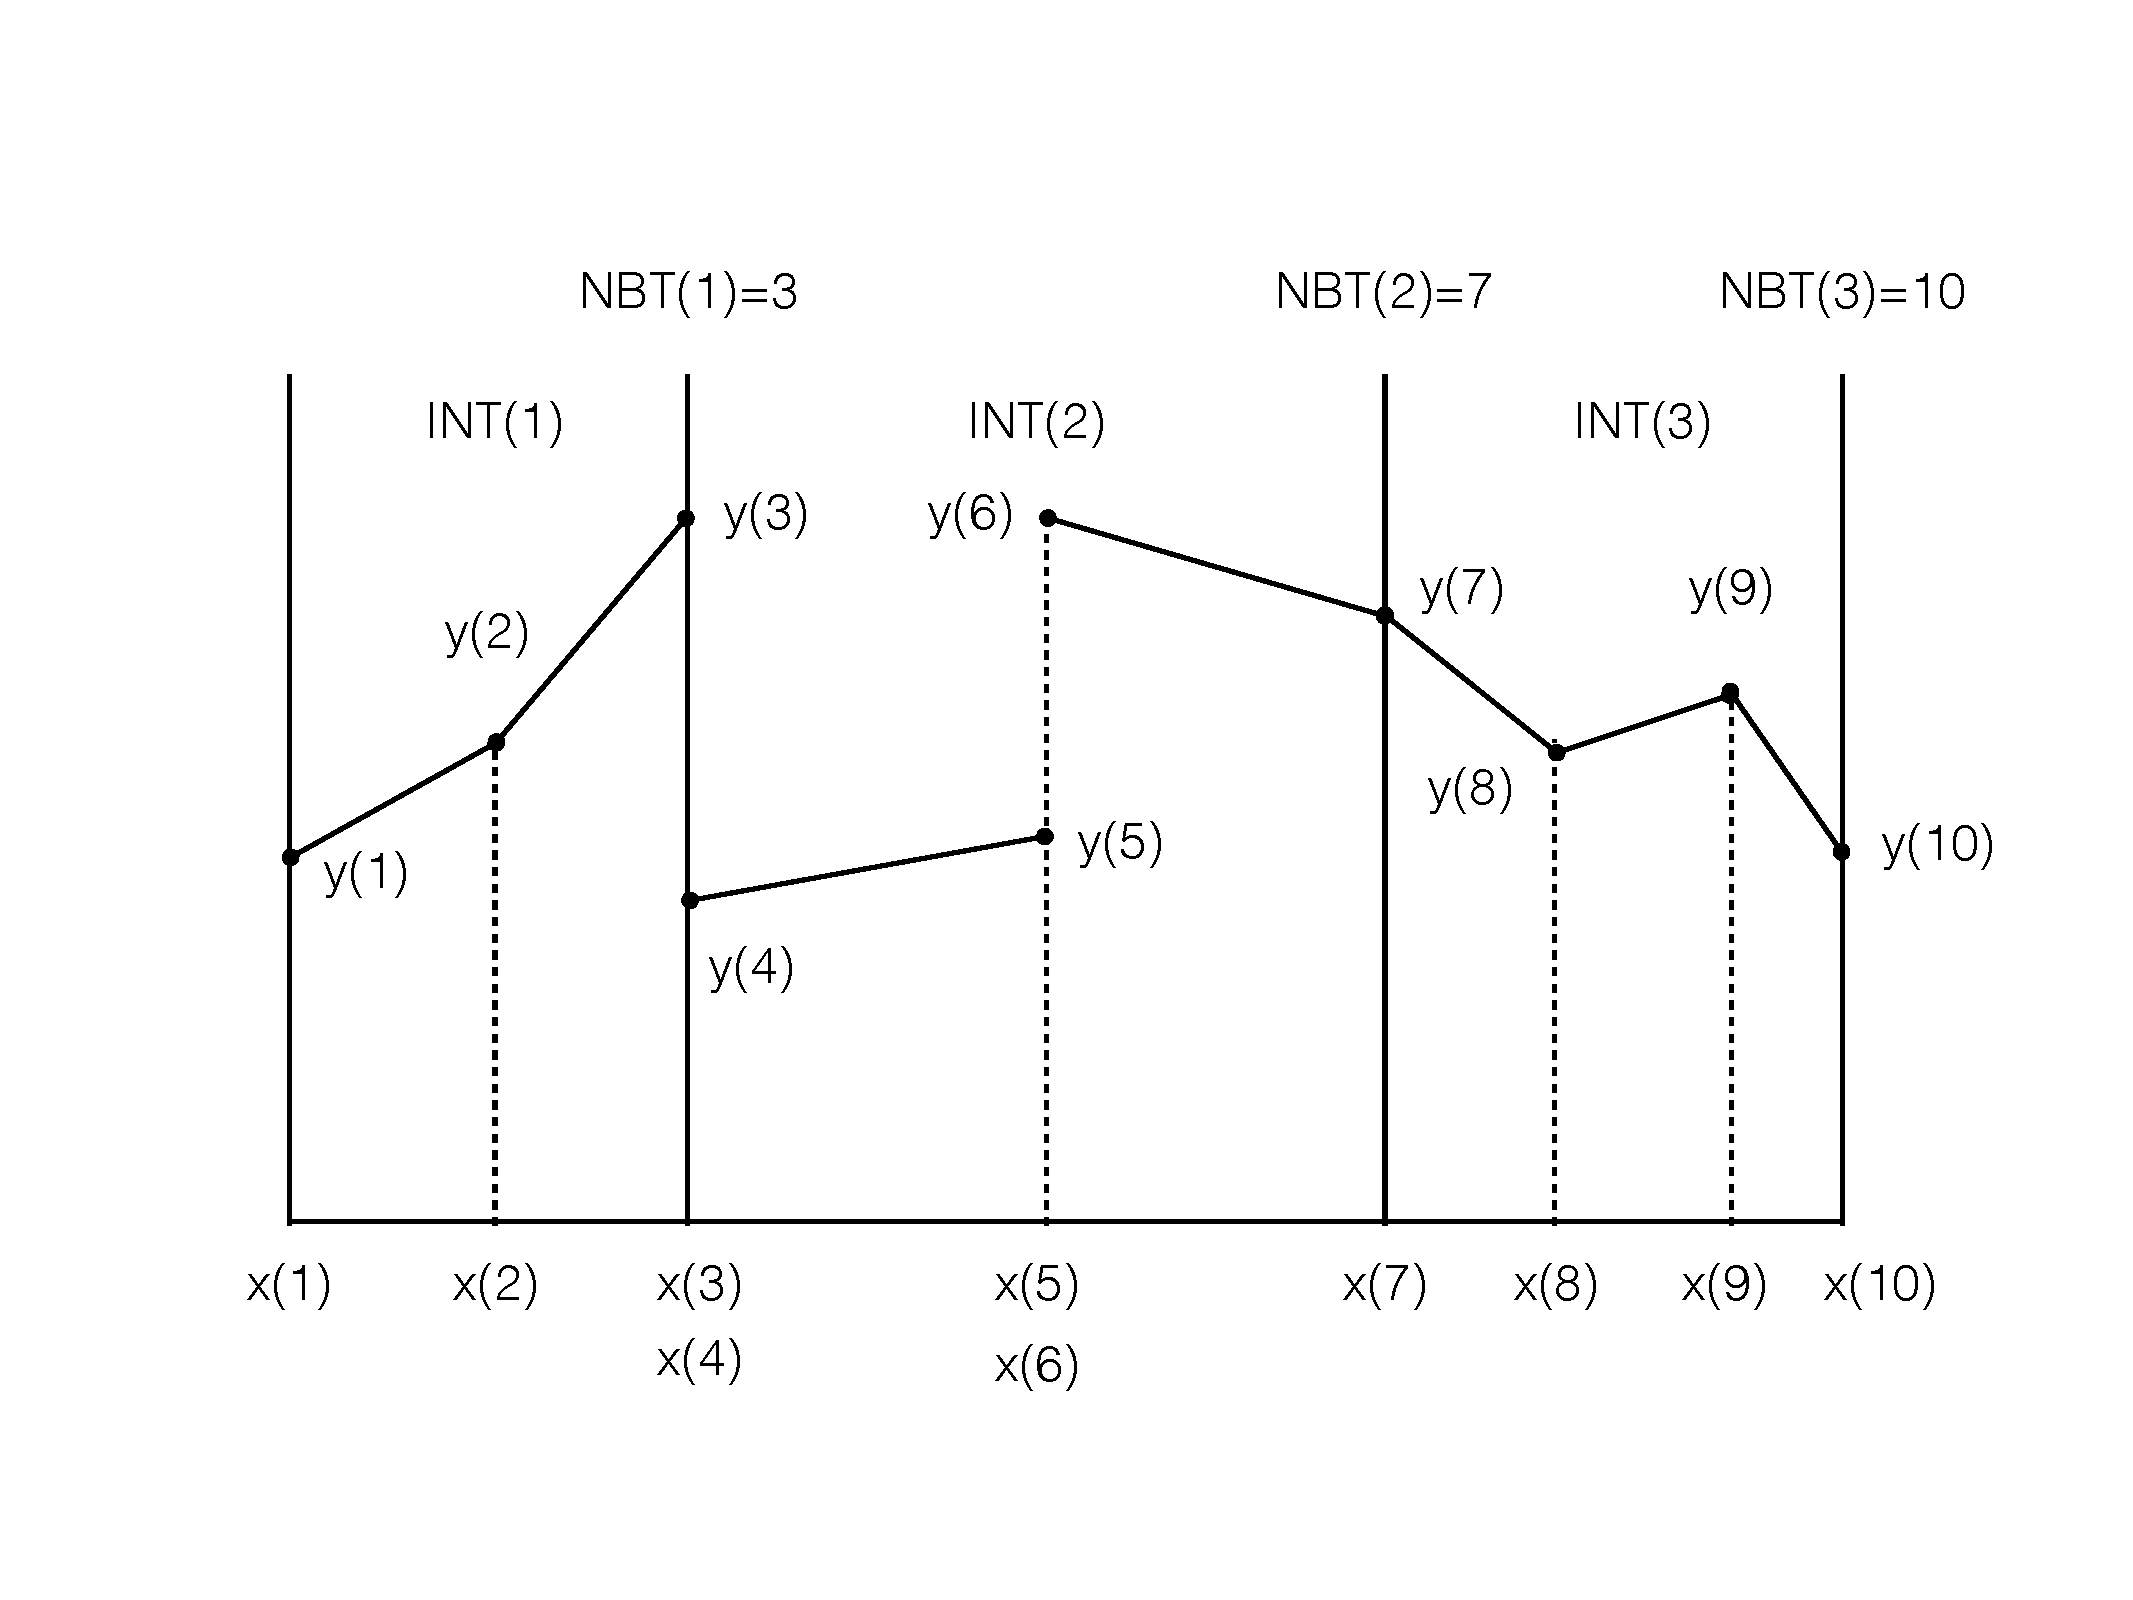
\includegraphics[scale=0.4]{./pics/endf-int-laws.pdf}
\end{center}
\caption{ \label{fig:endf-int-laws}
An example showing the ENDF interpolation rules of a function, the indices start from 1, but in C++ language, the indices start from 0}
\end{figure}
In the data structure, we have an public function`double evaluate(double x) const', which takes a given value $x$, and use the formula above to calculate the interpolated $y$.\\

\item{\em Polynomial function: } 
In the ENDF database, a function can be described by a polynomial with degree $n-1$ and coefficients $c_0, c_1, \dots, c_{n}$. The function value is evaluated by:
\begin{eqnarray}
y &=& \sum_{i=0}^{n-1}c_{i}\,x^i
\end{eqnarray}
The data structure for describing a polynomial function is given below:
\begin{verbatim}
struct ENDFPolynomialFunction {
    std::vector<double> coefficents;
    
    // Evaluate the polynomial function value at x
    double evaluate(double x) const;
};
\end{verbatim}
The `evaluate' function implements the evaluation of the function value at x.

\item{\em Function type: }
To specify whether a function is an ENDF interpolation or a polynomial, an enumeration is introduced as followed.
\begin{verbatim}
enum class ENDFFunctionType {
    INTERPOLATION = 1,
    POLYNOMIAL = 2
};
\end{verbatim}

\end{itemize}

\subsection{Fission Yield Data Structures}

The fission yield is an important property of the neutron data. For a fission nuclide, a fission can be prompt or delayed. Here, it discusses the data structures to describe the fission yield.

\begin{itemize}

\item{\em Fission spectrum: }
The fission spectrum describes the average number of neutron released as a function of the incident neutron energy. Such a function is denoted in $\bar{\nu}(E)$. For prompt fission, it is described as $\bar{\nu}_p(E)$, and for delayed fission, the sum is described as $\bar{\nu}_d(E)$. If there are $N$ precursor groups, the average number of neutron released from group $i$ is denoted as $\bar{\nu}_i(E)$, and
\begin{eqnarray}
\bar{\nu}_d(E) &=& \sum_{i=1}^{N}\bar{\nu}_i(E).
\end{eqnarray}
The average total fission neutron yield is given by $\bar{\nu}(E)$ and 
\begin{eqnarray}
\bar{\nu}(E) &=& \bar{\nu}_p(E) + \bar{\nu}_d(E).
\end{eqnarray}
The fission spectrum can be described either as an ENDF interpolation function or a polynomial function. So the data structure is listed as followed.
\begin{verbatim}
struct Spectrum {
    // The function type
    ENDFFunctionType type;
    // The data for interpolation function
    ENDFInterpolationFunction interpFunc;
    // The data for polynomial function
    ENDFPolynomialFunction polyFunc;
};
\end{verbatim}

\item{\em Precursor group: }
For precursor group $i$, there are the decay constant $\lambda_i$ and the group abundance $\alpha_i$. They can be either constant or energy dependent. So the precursors are described in the data structure as followed.
\begin{verbatim}
struct Precursor {
    // Decay constant, lambda
    double decayConst = 0.;
    // Decayed-group abundance, alpha
    double groupAbundance = 0.;
};
struct Precursors {
    // List of precursors
    std::vector<Precursor> precursors;
};
\end{verbatim}

\item{\em Neutron yield data: }
The neutron yield data is packed into a single data structure. The fission spectra are given in a C++ pointer. When the pointer is nullptr, then no such fission data is provided.
\begin{verbatim}
struct YieldData {
    ~YieldData();
    
    // Total neutron yield function
    Spectrum *total = nullptr;
    // Prompt neutron yield function
    Spectrum *prompt = nullptr;
    // Delayed neutron yield function
    Spectrum *delayed = nullptr;
    
    // Whether precursor is energy dependent
    bool isPrecursorEnergyDependent = false;
    // Energy independent precursors
    Precursors energyIndependentPrecursors;
    // Energy dependent precursors
    ENDFObjectInterpolationFunction< Precursors >
    energyDependentPrecursors;
};
\end{verbatim}

\end{itemize}

\subsection{Resonance Data Structure}

\begin{itemize}
\item
\end{itemize}

\subsection{Reaction Data Structure}
The reaction data structures taken from ENDF file 3 describe the `background' cross sections of reactions, which does not depend on the energy of the incident neutrons. The type of the reaction is determined by its `MT' number, whose definitions can be found in Table \ref{tab:mt-meaning}. The reaction cross sections are represented by the ENDF table with an `ENDFInterpolationFunction' data structure.
\begin{verbatim}
struct ReactionData {
    // Reaction number
    long   MT = -1;
    // Mass-difference Q value
    double QM = 0.;
    // Reaction Q value from the lowest energy state
    double QI = 0.;
    // Complex or "breakup" reaction flag
    long   LR = -1;
    // ENDF interpolated function for cross sections
    ENDFInterpolationFunction xsec;
};
\end{verbatim}

\begin{small}
\centering
\begin{longtable}{l l p{3.5cm} | l l p{3.5cm}}
MT & Symbol & Meaning & MT & Symbol & Meaning\\\hline
1 & (n,total) & total & 2 & (n,elastic) & elastic scattering\\\hline
3 & (n,inelastic) & inelastic scattering & 4 & (n,level) & level scattering\\\hline
5 & (n,other) & others & 11 & (n,2nd) & two neutrons plus one deuteron\\\hline 
16 & (n,2n) & two neutrons & 17 & (n,3n) & three neutrons\\\hline
18 & (n,fission) & fission & 19 & (n,f) & f \\\hline
20 & (n,nf) & one neutron and f & 21 & (n,2nf) & two neutrons and f\\\hline
22 & (n,na) & one neutron and one alpha & 23 & (n,n3a) & one neutron and three alphas\\\hline
24 & (n,2na) & two neutrons and one alpha & 25 & (n,3na) & three neutrons and one alpha\\\hline
28 & (n,np) & one neutron and one proton & 29 & (n,n2a) & one neutron and two alphas\\\hline
30 & (n,2n2a) & two neutrons and two alphas & 32 & (n,nd) & one neutron and one deuteron\\\hline
33 & (n,nt) & one neutron and one triton & 34 & (n,n3he) & one neutron and three helium\\\hline
35 & (n,nd2a) & one neutron, deuteron and two alphas & 36 & (n,nt2a) &  one neutron, triton and two alphas\\\hline
37 & (n,4n) & four neutrons & 38 & (n,3nf) & three neutrons and f\\\hline
41 & (n,2np) & two neutrons and one proton & 42 & (n,3np) & three neutrons and one proton\\\hline
44 & (n,n2p) & one neutron and two protons & 45 & (n,npa) & one neutron, proton and alpha\\\hline
$50+i$ & (n,n$i$) & $i$th level, $1\leq i\leq 40$ & 91 & (n,nc) & continuum scattering \\\hline
101 & (n,disappear) & & 102 & (n,gamma) & \\\hline
103 & (n,p) & & 104 & (n,d) & \\\hline
105 & (n,t) & & 106 & (n,3he) & \\\hline
107 & (n,a) & & 108 & (n,2a) & \\\hline
109 & (n,3a) & & 111 & (n,2p) & \\\hline
112 & (n,pa) & & 113 & (n,t2a) & \\\hline
114 & (n,d2a) & & 115 & (n,pd) & \\\hline
116 & (n,pt) & & 117 & (n,da) & \\\hline
$600+i$ & (n,p$i$) & $0\leq i\leq 48$ & 649 & (n,pc) & \\\hline
$650+i$ & (n,d$i$) & $0\leq i\leq 48$ & 699 & (n,dc) & \\\hline
$700+i$ & (n,t$i$) & $0\leq i\leq 48$ & 749 & (n,tc) & \\\hline
$750+i$ & (n,3he$i$) & $0\leq i\leq 48$ & 799 & (n,3hec) & \\\hline
$800+i$ & (n,a$i$) & $0\leq i\leq 48$ & 849 & (n,ac) & \\\hline
\caption{Meaning of the MT reaction number}
\label{tab:mt-meaning}
\end{longtable}
\end{small}

The relationship of the cross sections with different MT numbers is summarized in Table.

\subsection{Application Interfaces (APIs)}
